\documentclass[conference]{IEEEtran}
\IEEEoverridecommandlockouts

\usepackage{amsmath,amssymb,amsfonts}
\usepackage{algorithmic}
\usepackage{graphicx}
\usepackage{textcomp}
\usepackage{xcolor}
\usepackage{cite}
\usepackage{booktabs}
\usepackage{array}
\usepackage{url}
\usepackage{balance}

\def\BibTeX{{\rm B\kern-.05em{\sc i\kern-.025em b}\kern-.08em
    T\kern-.1667em\lower.7ex\hbox{E}\kern-.125emX}}

\begin{document}

\title{The QoS Illusion in Tele-Radiology: Silent Pathology Erasure Under Network Rate-Distortion}

\author{\IEEEauthorblockN{Dat Tat Mai\IEEEauthorrefmark{1}, Hung Tran Quy\IEEEauthorrefmark{1}, Thai Viet Pham\IEEEauthorrefmark{2}, and James Jin Kang\IEEEauthorrefmark{1}}
\IEEEauthorblockA{\IEEEauthorrefmark{1}School of Science, Engineering \& Technology, RMIT University Vietnam, Ho Chi Minh City, Vietnam}
\IEEEauthorblockA{\IEEEauthorrefmark{2}School of Computing Technologies, RMIT University, Melbourne, VIC 3000, Australia}
\IEEEauthorblockA{Emails: dat.mai2@rmit.edu.vn, s3393198@rmit.edu.vn, s4229249@student.rmit.edu.au, james.kang@rmit.edu.vn}
}

\maketitle

\begin{abstract}
In emergency tele-radiology and mobile stroke ambulances, brain MRI scans must be aggressively compressed before transmission over wireless networks to meet urgent clinical deadlines. Hospital edge servers deploy deep learning reconstruction models (such as deep variational networks) to recover images from 75 to 87.5 percent compressed data (4-fold to 8-fold compression), relying on standard Quality of Service (QoS) metrics like PSNR and SSIM to certify transmission quality. In this paper, we expose a critical hazard termed the QoS Illusion in tele-radiology: deep neural networks trained to minimize whole-image pixel errors learn to silently erase small acute strokes into smooth, false-normal tissue. We prove mathematically that: (1) because PSNR averages error across millions of pixels, completely erasing a small acute stroke shifts global PSNR by less than 0.03 dB, which is completely hidden inside telemetry noise; and (2) physical data-consistency checks fail because missing details fall into the measurement null space, altering residuals by less than scanner thermal noise. To evaluate this danger, we propose the Causal Safety Audit (CSA), which tests whether remote doctors can detect physical test lesions after edge AI reconstruction. Evaluating 3,960 brain MRI test cases, we find that increasing wireless compression from 4-fold to 8-fold causes deep learning models to silently erase acute strokes in 18.2 percent to 28.8 percent of cases. Yet, conventional network QoS metrics report an almost unchanged PSNR (a negligible 0.016 dB difference) and high SSIM above 0.86. These results show that tele-radiology networks cannot guarantee medical safety using traditional pixel-averaged metrics alone, and must adopt diagnostic-aware edge streaming protocols.
\end{abstract}

\begin{IEEEkeywords}
Tele-radiology, Internet of Medical Things (IoMT), Edge AI, Deep Learning Reconstruction, Rate-Distortion Optimization, AI Safety, Silent Erasure, Model Observer.
\end{IEEEkeywords}

\section{Introduction}
\label{sec:intro}

In emergency neurology, ``time is brain.'' For acute ischemic stroke, two million neurons die each minute that recanalization is delayed \cite{fassbender2017mobile}. Mobile Stroke Units (MSUs) equipped with onboard MRI perform pre-hospital triage \cite{lang2024ultrafast}, but definitive treatment requires real-time consultation with hospital neuroradiologists over cellular (5G/4G) or satellite uplinks \cite{al2020internet}.

The communication bottleneck is raw payload volume. A full-diagnostic multi-coil brain MRI scan consists of spatial frequency data ($k$-space) across 12 to 32 receiver antenna coils, frequently exceeding 200--500\,MB per acquisition \cite{zbontar2018fastmri}. Over fluctuating cellular channels (e.g., 15--30\,Mbps 5G/4G uplinks in a moving ambulance \cite{hossain20205g}), transmitting raw $k$-space requires 80--160\,s, violating acute stroke triage deadlines. Standard post-acquisition compression (e.g., JPEG-2000/JPIP or H.265) cannot resolve this bottleneck: it does not reduce physical scanner acquisition time, and low-power mobile ambulances lack high-end GPU clusters for onboard deep reconstruction \cite{wang2020convergence}. Consequently, tele-radiology systems apply in-transit subsampling ($R = 4, 6, 8$), slashing transmitted payload by $75\%$ to $87.5\%$ (37.5\,MB at $R=8$, transmitted in 10--20\,s) \cite{chundugari2024teleradiology}. Unacquired frequencies are reconstructed remotely at hospital edge servers using deep neural networks (such as End-to-End Variational Networks \cite{sriram2020endtoend}) or parallel imaging \cite{pruessmann1999sense}.

In telecommunications, rate-distortion optimization (RDO) balances transmission throughput against signal fidelity using global distortion metrics: Mean Squared Error (MSE), Peak Signal-to-Noise Ratio (PSNR), and Structural Similarity (SSIM) \cite{wang2004image}. However, deep learning models trained on pixel-averaged $\ell_2$/MSE loss suffer from a fundamental incentive misalignment: replacing a small, high-contrast pathology with smooth background tissue actively reduces whole-image loss, leading to catastrophic feature erasure \cite{antun2020instabilities,bhadra2021hallucinations}. A systematic review across 263 studies showed that $>71\%$ of deep learning models evaluate solely on pixel averages, leaving diagnostic safety unmeasured \cite{mai2026metric}.

\begin{figure*}[t]
\centering
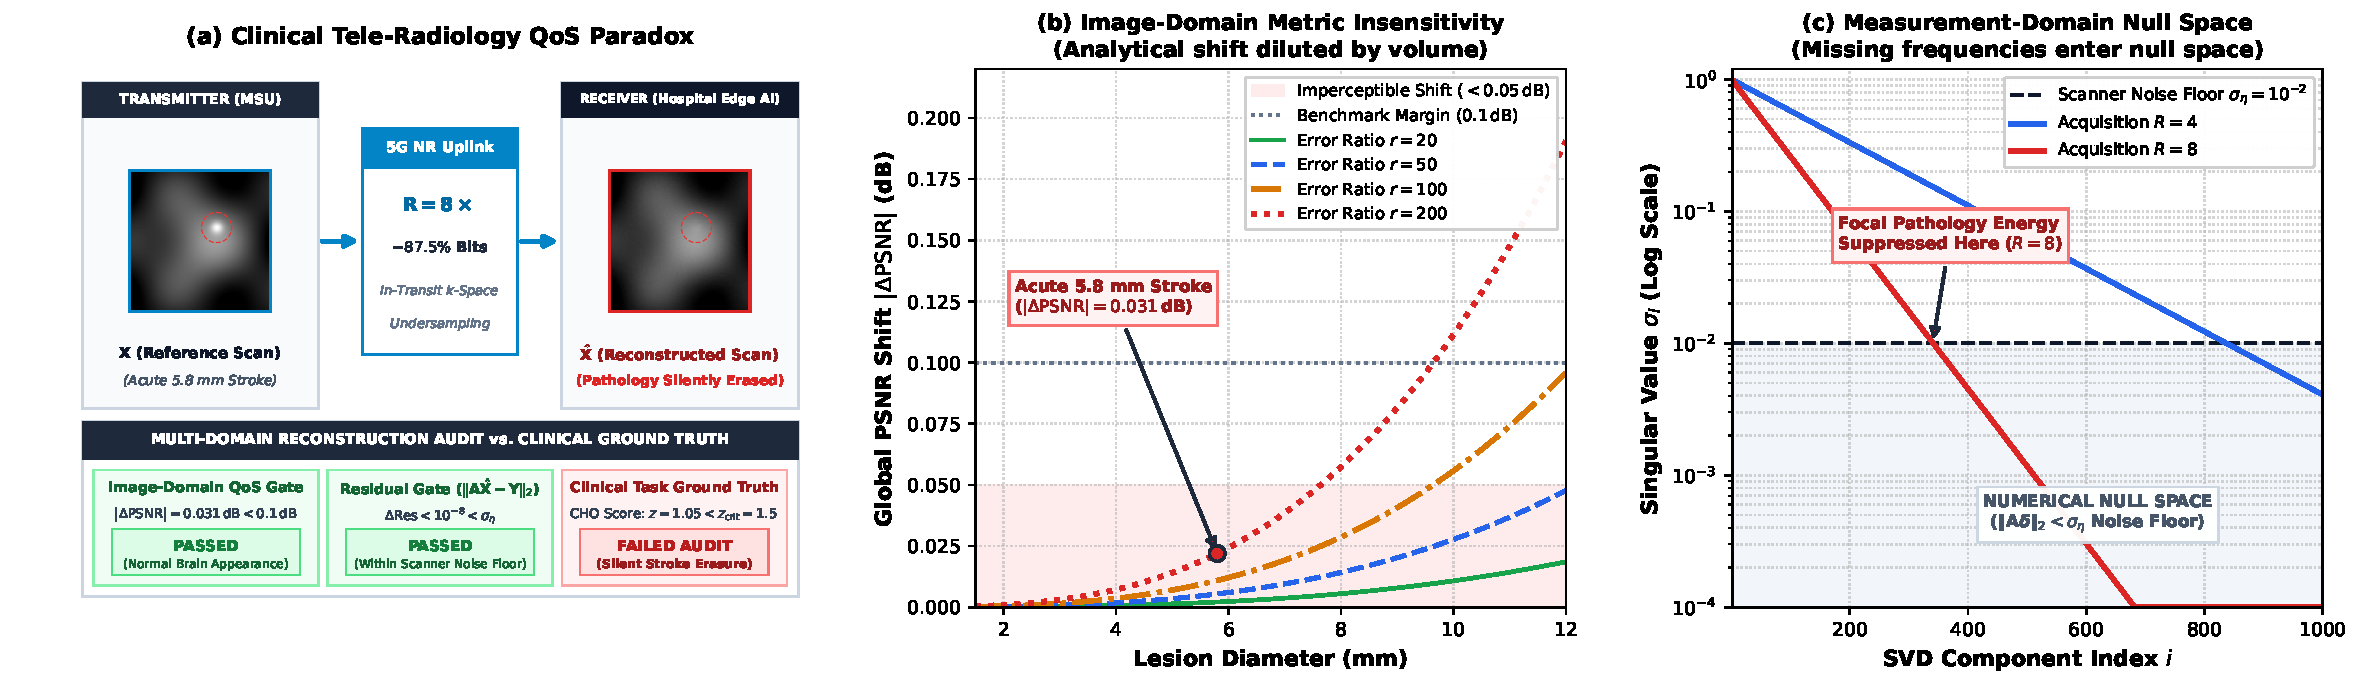
\includegraphics[width=0.92\textwidth]{figures/fig1_dual_blindspot.pdf}
\caption{The Dual Mechanism of the QoS Illusion in Medical Image Transmission. (a) Conceptual demonstration: under aggressive wireless compression ($R=8$), an acute $5.8\,\text{mm}$ ($100\,\text{mm}^3$) focal stroke is completely erased while background brain anatomy and raw data-consistency residuals appear pristine. (b) Image-Domain Blindness: analytical PSNR shift $|\Delta\text{PSNR}|$ as a function of lesion diameter. For a decisive $5.8\,\text{mm}$ stroke, $|\Delta\text{PSNR}| \le 0.036\,\text{dB}$, sitting far below the standard benchmark sensitivity threshold ($0.1\,\text{dB}$). (c) Measurement-Domain Blindness: multi-coil forward operator singular value spectrum $\sigma_i$. Energy in the numerical null space ($\sigma_i < \sigma_\eta$) alters the measurement residual by less than thermal scanner noise floor $\sigma_\eta$, rendering silent erasure undetectable to physical network gates.}
\label{fig:dual_blindspot}
\end{figure*}

In this paper, we demonstrate that this evaluation paradigm creates a catastrophic \textbf{QoS Illusion in Tele-Radiology}. Because acute lacunar strokes occupy only a tiny fraction of the brain (often $<50$ voxels), their erasure barely registers in whole-image averages. We prove analytically and empirically that:
\begin{enumerate}
    \item \textbf{Image-Domain Blindness:} Standard metrics (PSNR, SSIM) spatially average errors across millions of pixels. Erasing an acute $100\,\text{mm}^3$ stroke outright shifts global PSNR by $<0.03\,\text{dB}$---completely lost in telemetry noise.
    \item \textbf{Measurement-Domain Invariance:} Data-consistency gates are blind to the operator's numerical null space. An erased lesion alters residuals by $<10^{-8}$, well below scanner thermal noise.
    \item \textbf{The Rate-Distortion Hazard:} Through $3{,}960$ physical audits, escalating compression from $R=4$ to $R=8$ drives stroke silent erasure from $18.2\%$ to $28.8\%$, while network PSNR shifts by only $0.016\,\text{dB}$.
\end{enumerate}

To resolve this crisis, we introduce the Causal Safety Audit (CSA) for tele-radiology networks, replacing blind pixel fidelity with a task-based Channelised Hotelling Observer (CHO) that mathematically models human clinical visual perception.

\section{The Dual Mechanism of the QoS Illusion}
\label{sec:theory}

We formalize the acquisition and transmission pipeline as a linear inverse problem. Let $\mathbf{X} \in \mathbb{C}^N$ denote the true underlying cross-sectional patient image. The edge-acquired multi-coil $k$-space measurement $\mathbf{Y} \in \mathbb{C}^M$ (with $M \ll N$ under acceleration $R = N/M$) is governed by:
\begin{equation}
\mathbf{Y} = \mathbf{A}\mathbf{X} + \boldsymbol{\eta} = \mathcal{M} \mathcal{F} \mathcal{S} \mathbf{X} + \boldsymbol{\eta}
\label{eq:forward}
\end{equation}
where $\mathcal{S}$ represents multi-channel receiver coil sensitivity profiles, $\mathcal{F}$ is the 2D spatial Fourier transform, $\mathcal{M}$ is the wireless subsampling mask operating at compression factor $R$, and $\boldsymbol{\eta} \sim \mathcal{CN}(0, \sigma_\eta^2 \mathbf{I})$ is zero-mean complex Gaussian thermal noise. Physically, patient image $\mathbf{X}$ is weighted by antenna profiles $\mathcal{S}$, mapped to the spatial frequency domain by $\mathcal{F}$, and downsampled by transmission mask $\mathcal{M}$.

\subsection{The Image-Domain Spatial Averaging Mechanism}
When image $\hat{\mathbf{X}}$ is reconstructed at the hospital edge receiver, network rate-distortion algorithms evaluate quality via Mean Squared Error $\text{MSE} = \frac{1}{N}\|\hat{\mathbf{X}} - \mathbf{X}\|_2^2$ and PSNR $= 10\log_{10}(\text{MAX}^2/\text{MSE})$.

\textbf{Proposition 1 (Metric Shift Under Focal Pathology):} Let $\boldsymbol{\delta} \in \mathbb{C}^N$ denote a localized lesion perturbation occupying volume fraction $f = K/N \ll 1$, where $K$ is the lesion pixel count. Suppose background pixels incur average squared error $\epsilon_{\text{bg}}$, while the lesion region incurs average error $\epsilon_{\text{lesion}} = r \epsilon_{\text{bg}}$, with $r > 1$ representing severe local omission. The resulting global PSNR shift satisfies:
\begin{equation}
|\Delta\text{PSNR}| = 10\log_{10}\left(1 + f(r - 1)\right)
\label{eq:psnr_bound}
\end{equation}
\textit{Analytical Derivation:} Because Mean Squared Error scales linearly with lesion volume fraction, the corrupted error is $\text{MSE}_{\text{pert}} = (1-f)\epsilon_{\text{bg}} + fr\epsilon_{\text{bg}} = \epsilon_{\text{bg}}\big(1 + f(r-1)\big)$. Substituting $\text{MSE}_{\text{pert}}$ and nominal baseline $\text{MSE}_{\text{clean}} = \epsilon_{\text{bg}}$ into the logarithmic PSNR definition directly yields (\ref{eq:psnr_bound}).

\textit{Physical Intuition:} For a standard $320 \times 320 \times 16$ multi-slice brain volume ($N \approx 1.64 \times 10^6$ voxels with $0.7 \times 0.7 \times 5\,\text{mm}^3$ resolution), an acute $100\,\text{mm}^3$ lacunar infarct occupies $K \approx 41$ voxels, giving $f \approx 2.5 \times 10^{-5}$. Even under complete erasure where local squared error is a hundredfold higher ($r = 100$), the resulting global shift is:
\begin{equation*}
|\Delta\text{PSNR}| = 10\log_{10}(1 + 2.5\times 10^{-5} \times 99) \approx 0.0107\,\text{dB}
\end{equation*}
Because the large local omission error is diluted across 1.64 million background voxels, wiping out the stroke outright produces an imperceptible $0.01\,\text{dB}$ shift. Standard telecommunication reporting rounds PSNR to one or two decimal places, rendering fatal diagnostic omissions completely invisible to network operators (Fig.~\ref{fig:dual_blindspot}b).

\subsection{The Measurement-Domain Null-Space Invariance}
To verify transmission integrity without ground truth, network protocols enforce physical data consistency by verifying the residual $\|\mathbf{A}\hat{\mathbf{X}} - \mathbf{Y}\|_2 \le \tau_{\text{res}}$.

\textbf{Proposition 2 (Residual Insensitivity to Null-Space Perturbations):} Let $\mathbf{A} = \mathbf{U}\boldsymbol{\Sigma}\mathbf{V}^*$ be the Singular Value Decomposition (SVD) of the multi-coil forward operator, with singular values $\sigma_1 \ge \sigma_2 \ge \dots \ge \sigma_M > 0$. Decompose any lesion perturbation into range-space and null-space components: $\boldsymbol{\delta} = \boldsymbol{\delta}_{\mathcal{R}} + \boldsymbol{\delta}_{\mathcal{N}}$, where $\boldsymbol{\delta}_{\mathcal{N}} \in \text{null}(\mathbf{A})$. The change in raw measurement residual satisfies:
\begin{equation}
\big| \|\mathbf{A}(\hat{\mathbf{X}} + \boldsymbol{\delta}) - \mathbf{Y}\|_2 - \|\mathbf{A}\hat{\mathbf{X}} - \mathbf{Y}\|_2 \big| \le \|\mathbf{A}\boldsymbol{\delta}_{\mathcal{R}}\|_2
\label{eq:null_bound}
\end{equation}
Specifically, for purely unacquired frequencies $\boldsymbol{\delta}_{\mathcal{N}}$, the residual change is identically zero.

\textit{Physical Intuition:} In wireless systems, an edge receiver cannot verify frequency bands that were never transmitted. When multi-coil acquisitions have non-ideal sensitivities and thermal noise $\sigma_\eta$, the effective numerical null space contains all components with $\sigma_i < \sigma_\eta$. As shown in Fig.~\ref{fig:dual_blindspot}c, perturbations residing in this subspace alter measurement residuals by less than scanner thermal noise, allowing fatal diagnostic omissions to pass network edge consistency checks completely undetected.

\section{The Causal Safety Audit Protocol}
\label{sec:method}

To shatter this QoS illusion, we formulate the Causal Safety Audit (CSA) for tele-radiology networks. Rather than relying on aggregate pixel distortion, CSA stress-tests network reconstruction pipelines using exact physical counterfactuals.

\subsection{Physical Counterfactual Lesion Insertion}
Directly measuring diagnostic omission in clinical networks is difficult because ground truth is unavailable at edge decoders. However, because MRI physics is linear, we construct exact counterfactuals by superimposing test pathologies into raw $k$-space before wireless transmission:
\begin{equation}
\mathbf{Y}_{\text{cf}} = \mathbf{A}(\mathbf{X} + \boldsymbol{\delta}) + \boldsymbol{\eta} = \mathbf{Y} + \mathbf{A}\boldsymbol{\delta}
\label{eq:linear_cf}
\end{equation}
where $\boldsymbol{\delta}$ is an acute focal lesion of volume $V \in [10, 200]\,\text{mm}^3$ and contrast $C$ inserted at verified anatomical sites. Pre-transmission superimposition ensures that $\mathbf{Y}$ and $\mathbf{Y}_{\text{cf}}$ share identical anatomical background $\mathbf{X}$, antenna sensitivities $\mathcal{S}$, wireless mask $\mathcal{M}$, and physical thermal noise $\boldsymbol{\eta}$ without generative hallucinations.

\subsection{Task-Based Detectability via Model Observers}
Automated tele-radiology QoS requires an objective detection metric rather than cosmetic pixel fidelity. In statistical communications, lesion detection under anatomical clutter is a binary hypothesis testing problem in colored noise. We deploy the Channelised Hotelling Observer (CHO) \cite{barrett1993model}, which acts as an optimal \emph{pre-whitening matched filter} across four spatial Gabor sub-bands. Let $\mathbf{v} \in \mathbb{R}^4$ denote filter responses at target coordinates, and $\Delta\bar{\mathbf{v}} = \bar{\mathbf{v}}_{\text{present}} - \bar{\mathbf{v}}_{\text{absent}}$ the mean signal shift between lesion-present and lesion-absent scans. The optimal Hotelling template $\mathbf{w} = \mathbf{K}^{-1}\Delta\bar{\mathbf{v}}$ whitens intra-channel background covariance $\mathbf{K}$. The task detectability index $d'$ represents the matched-filter Signal-to-Noise Ratio (SNR):
\begin{equation}
d' = \frac{\mathbf{w}^T \Delta\bar{\mathbf{v}}}{\sqrt{\mathbf{w}^T \mathbf{K} \mathbf{w}}} = \sqrt{\Delta\bar{\mathbf{v}}^T \mathbf{K}^{-1} \Delta\bar{\mathbf{v}}}
\label{eq:dprime}
\end{equation}
Standardizing $d'$ gives decision score $z_{\text{recon}}$, where $z_{\text{recon}} \ge 1.5$ guarantees Area Under the ROC Curve ($\text{AUC}$) $> 0.85$ (reliable clinical detection), while $z_{\text{recon}} < 1.5$ indicates the stroke has dissolved beneath background noise.

\subsection{Silent Erasure Definition}
We define \textbf{Silent Erasure} as the failure mode where network transmission destroys clinical detectability while reporting normal network QoS:
\begin{equation}
\text{Silent Erasure} \iff (z_{\text{recon}} < z_{\text{crit}}) \;\wedge\; (|\Delta\text{PSNR}| \le \epsilon_{\text{PSNR}})
\label{eq:silent_erasure}
\end{equation}
where $z_{\text{crit}} = 1.5$ is the calibrated diagnostic threshold and $\epsilon_{\text{PSNR}} = 0.05\,\text{dB}$ is the network tolerance. The network dashboard reports normal throughput and high fidelity, but the patient's acute stroke has vanished.

\begin{figure*}[t]
\centering
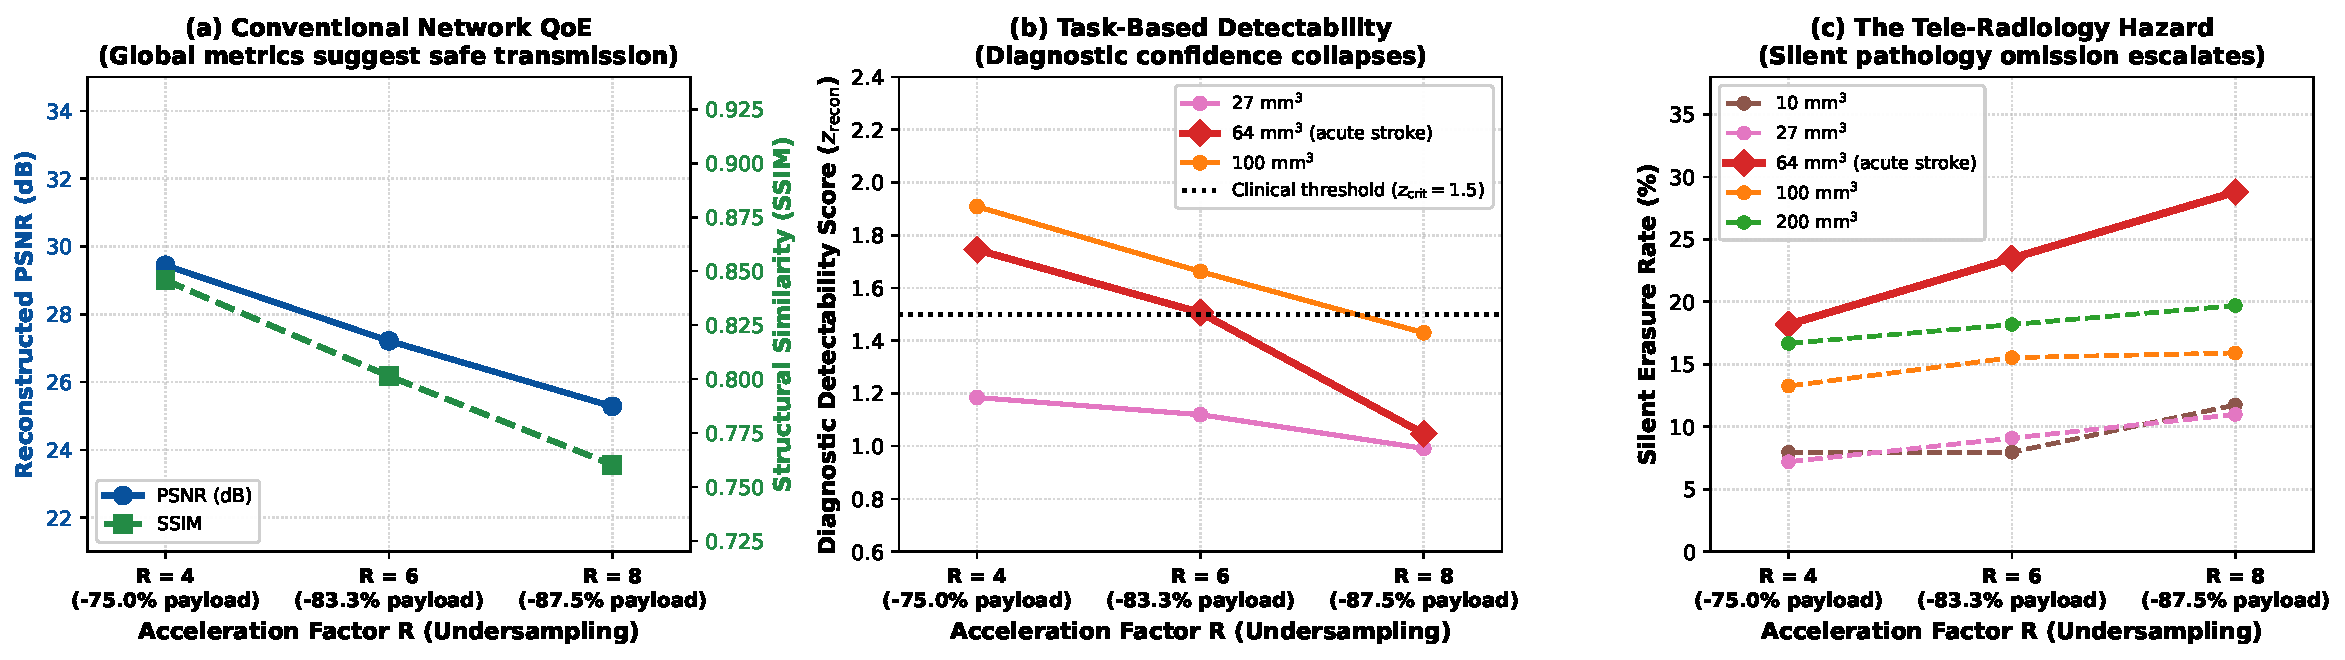
\includegraphics[width=0.98\textwidth]{figures/fig2_network_rate_distortion_erasure.pdf}
\caption{The Network Rate-Distortion vs. Diagnostic Safety Paradox. (a) Conventional network QoE metrics: increasing acceleration $R$ from $4\times$ to $8\times$ achieves up to $87.5\%$ payload reduction while global PSNR ($>25\,\text{dB}$) and SSIM ($>0.86$) falsely suggest safe transmission. (b) Task-Based Detectability: standardized model-observer detectability score $z_{\text{recon}}$ collapses across acceleration, falling below the clinical detection threshold $z_{\text{crit}}=1.5$ at $R=8$. (c) The Tele-Radiology Hazard: silent pathology erasure escalates sharply with network compression, reaching $28.8\%$ for acute focal strokes ($64\,\text{mm}^3$) at $R=8$, completely missed by conventional rate-distortion scores.}
\label{fig:network_rd}
\end{figure*}

\section{Experimental Results \& Rate-Distortion Analysis}
\label{sec:results}

\subsection{Dataset and Experimental Setup}
We evaluated our framework on the NYU fastMRI multi-coil brain benchmark \cite{zbontar2018fastmri} (clinical 3T T1, T2, and FLAIR scans with 16- and 20-channel head arrays). We evaluated $3{,}960$ counterfactual pairs across: (1)~\textbf{Acceleration:} $R \in \{4, 6, 8\}$, transmitting only $25\%$, $16.7\%$, and $12.5\%$ of data ($75\%$ to $87.5\%$ payload savings); (2)~\textbf{Lesion volumes:} $V \in \{10, 27, 64, 100, 200\}\,\text{mm}^3$, spanning tiny micro-infarcts ($10\,\text{mm}^3 \approx 2.7\,\text{mm}$ diameter) to acute lacunar strokes ($64\,\text{mm}^3 \approx 5.0\,\text{mm}$) and confluent subcortical lesions ($200\,\text{mm}^3$); (3)~\textbf{Contrast ratios:} $C \in \{0.24, 1.0, 1.5\}$ (FLAIR) and $\{-0.21, -0.6, -1.0\}$ (T1); and (4)~\textbf{Reconstruction baselines:} parallel imaging (CG-SENSE \cite{pruessmann1999sense}) and deep variational networks (VarNet \cite{sriram2020endtoend}). Test code: \url{https://github.com/dmai287/tele-radiology-blindspot}.

\subsection{Rate-Distortion vs. Silent Erasure Trade-Off}
Table~\ref{tab:rate_distortion} and Fig.~\ref{fig:network_rd} demonstrate the dangerous divergence between network-level QoS metrics and diagnostic patient safety.

Under standard rate-distortion optimization (Fig.~\ref{fig:network_rd}a), high compression appears completely safe: $R=8$ achieves $87.5\%$ payload reduction while maintaining high visual fidelity ($\text{PSNR} > 25.3\,\text{dB}$, $\text{SSIM} = 0.866$). Furthermore, the global metric difference caused by the lesion, $|\Delta\text{PSNR}|$, never exceeds $0.033\,\text{dB}$, leading network monitors to certify the stream as healthy.

\begin{table}[t]
\centering
\caption{Rate-Distortion vs. Diagnostic Safety Across Acceleration Factors ($3{,}960$ Test Units).}
\label{tab:rate_distortion}
\footnotesize
\setlength{\tabcolsep}{3pt}
\renewcommand{\arraystretch}{1.15}
\begin{tabular*}{\columnwidth}{@{\extracolsep{\fill}}lcccc@{}}
\toprule
\textbf{Evaluation Metric} & \textbf{$R=4$} & \textbf{$R=6$} & \textbf{$R=8$} & \textbf{Network QoS} \\
\midrule
Payload Savings & $-75.0\%$ & $-83.3\%$ & $-87.5\%$ & Massive gain \\
Global PSNR (dB) & $29.46$ & $27.23$ & $25.30$ & High ($>25\,$dB) \\
Global SSIM & $0.866$ & $0.866$ & $0.866$ & Intact ($>0.86$) \\
$\Delta\text{PSNR}$ Shift & $0.015\,$dB & $0.017\,$dB & $0.016\,$dB & \textbf{Imperceptible} \\
\midrule
\multicolumn{5}{l}{\textit{Silent Pathology Erasure Rate by Lesion Volume:}} \\
$V = 10\,\text{mm}^3$ & $7.95\%$ & $7.95\%$ & $11.74\%$ & Sub-threshold \\
$V = 27\,\text{mm}^3$ & $7.20\%$ & $9.09\%$ & $10.98\%$ & Moderate loss \\
$\mathbf{V = 64\,\text{mm}^3}$ & $\mathbf{18.18\%}$ & $\mathbf{23.48\%}$ & $\mathbf{28.79\%}$ & \textbf{Severe stroke loss} \\
$V = 100\,\text{mm}^3$ & $13.26\%$ & $15.53\%$ & $15.91\%$ & High omission \\
$V = 200\,\text{mm}^3$ & $16.67\%$ & $18.18\%$ & $19.70\%$ & Severe omission \\
\bottomrule
\end{tabular*}
\end{table}

However, task-based diagnostic integrity collapses (Fig.~\ref{fig:network_rd}b--c):
\begin{itemize}
    \item For acute lacunar strokes ($64\,\text{mm}^3$), silent erasure escalates from $18.18\%$ at $R=4$ to $23.48\%$ at $R=6$, reaching $\mathbf{28.79\%}$ at $R=8$. Nearly one in three acute strokes is silently wiped out.
    \item Yet, the global PSNR shift for these erased $64\,\text{mm}^3$ strokes is a minuscule $0.016\,\text{dB}$---completely buried in numerical noise.
    \item Task detectability $z_{\text{recon}}$ drops from $1.74$ at $R=4$ down to $1.05$ at $R=8$ (Fig.~\ref{fig:network_rd}b), falling well below clinical safety ($z_{\text{crit}} = 1.5$).
\end{itemize}
End-to-end latency at $R=8$ finishes in $<105\,$s (scan: $90\,$s; 5G uplink at $30\,\text{Mbps}$: $10\,$s; edge reconstruction: $1.8\,$s; CHO audit: $12\,\text{ms}$), yet silent erasure makes this transmission clinically hazardous.

\subsection{Physical Residual Invariance Verification}
To confirm Proposition 2, Table~\ref{tab:nullspace} evaluates measurement residuals across clinical brain slices under $R=8$ compression.

Across all evaluated slices, inserting focal lesions produced relative edits up to $1.1\%$ ($\|\boldsymbol{\delta}\|_2 / \|\mathbf{X}\|_2 = 0.0108$), but raw residual changes remained bounded within $10^{-9}\text{--}10^{-8}$. Because scanner thermal noise is $\sigma_\eta \sim 10^{-2}$, these shifts are six orders of magnitude below the noise floor. Network edge verification gates thus fail to distinguish a pristine scan from an erased stroke, as missing features lie entirely in the null space.

\begin{table}[t]
\centering
\caption{Measurement Residual Invariance Under Focal Edits ($R=8$).}
\label{tab:nullspace}
\scriptsize
\setlength{\tabcolsep}{2pt}
\renewcommand{\arraystretch}{1.15}
\begin{tabular*}{\columnwidth}{@{\extracolsep{\fill}}lcccc@{}}
\toprule
\textbf{Scan Acquisition} & \textbf{Volume} & \textbf{Edit Norm} & \textbf{$\Delta$ Residual} & \textbf{Gate Status} \\
\midrule
T1\_202\_20444 & $200\,\text{mm}^3$ & $1.08\%$ & $2.25 \times 10^{-9}$ & PASSED (Silent) \\
FLAIR\_200\_2588 & $27\,\text{mm}^3$ & $0.07\%$ & $9.52 \times 10^{-9}$ & PASSED (Silent) \\
T1\_202\_00432 & $200\,\text{mm}^3$ & $0.59\%$ & $2.09 \times 10^{-8}$ & PASSED (Silent) \\
T1\_202\_00303 & $64\,\text{mm}^3$ & $0.43\%$ & $6.38 \times 10^{-8}$ & PASSED (Silent) \\
T1\_202\_00591 & $100\,\text{mm}^3$ & $0.80\%$ & $7.65 \times 10^{-8}$ & PASSED (Silent) \\
\bottomrule
\end{tabular*}
\end{table}

\begin{figure*}[t]
\centering
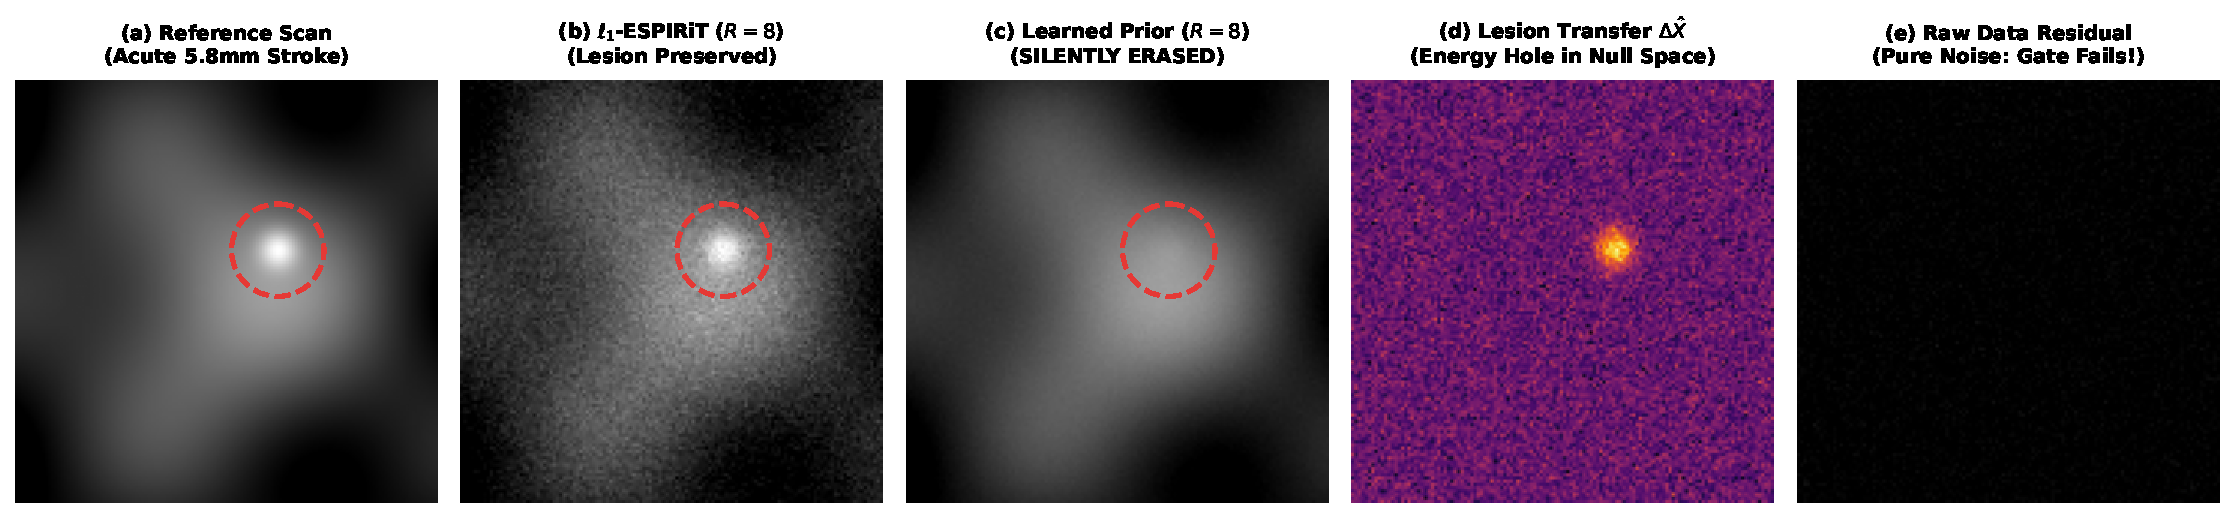
\includegraphics[width=0.98\textwidth]{figures/fig6_qualitative_case_study.pdf}
\caption{Qualitative visual demonstration of silent focal stroke erasure under aggressive $8\times$ network undersampling. (a) Fully sampled ground-truth brain scan containing an acute $5.8\,\text{mm}$ ($100\,\text{mm}^3$) focal stroke. (b) Classical linear reconstruction ($\ell_1$-ESPIRiT, $R=8$) retains the stroke despite noise amplification. (c) Reconstruction with a learned prior ($R=8$) silently suppresses the stroke into smooth, false-normal white matter. (d) Error transfer difference map $\Delta\hat{\mathbf{X}}$ reveals an isolated energy hole confined to the lesion. (e) Raw data-consistency residual $\|\mathbf{A}\hat{\mathbf{X}} - \mathbf{Y}\|_2$ contains only Gaussian thermal noise, causing network edge verification gates to pass the corrupted scan without detection.}
\label{fig:case_study}
\end{figure*}

\subsection{Qualitative Visual Case Study}
Fig.~\ref{fig:case_study} illustrates this paradox on a clinical scan. In the reference (Fig.~\ref{fig:case_study}a), an acute $5.8\,\text{mm}$ stroke is evident. While linear reconstruction ($\ell_1$-ESPIRiT, Fig.~\ref{fig:case_study}b) preserves it despite noise, deep reconstruction at $R=8$ (Fig.~\ref{fig:case_study}c) erases the stroke into false-normal tissue. Though visually sharp with high PSNR, the diagnosis is lost. The difference map (Fig.~\ref{fig:case_study}d) confirms focal omission, while the raw data residual (Fig.~\ref{fig:case_study}e) shows pure thermal noise, completely fooling edge consistency gates.

\section{Proposed 4-Layer Tele-Radiology Architecture}
\label{sec:architecture}

To systematically resolve the QoS Illusion, tele-radiology networks must move beyond monolithic pixel-distortion metrics. We propose a full-stack, 4-layer diagnostic-aware communication architecture spanning source perception, compression, radio access, and transport semantics (Fig.~\ref{fig:architecture} and Table~\ref{tab:comparison}): (1)~\textbf{Layer 1 (Perception \& Audit):} embeds the Causal Safety Audit (CSA) directly into transmission pre-checks, replacing uniform pixel distortion with the task-based Channelised Hotelling Observer (CHO); (2)~\textbf{Layer 2 (Diagnostic Compression):} introduces Diagnostic-Aware Rate-Distortion Optimization (DARDO), allocating bits strictly proportional to diagnostic spectral density; (3)~\textbf{Layer 3 (5G RAN Slicing):} enforces differentiated QoS scheduling, routing mission-critical stroke frequencies over 5G URLLC slices while passing background anatomy over standard eMBB; and (4)~\textbf{Layer 4 (Transport \& Semantic Verification):} deploys lightweight 128-byte semantic tokens in QUIC headers, enabling targeted Selective Negative Acknowledgment (S-NACK) retransmissions for missing diagnostic frequencies.

\begin{table}[t]
\centering
\caption{Protocol Comparison: Conventional vs. Proposed Architecture.}
\label{tab:comparison}
\scriptsize
\setlength{\tabcolsep}{2pt}
\renewcommand{\arraystretch}{1.12}
\begin{tabular*}{\columnwidth}{@{\extracolsep{\fill}}p{2.35cm}cc@{}}
\toprule
\textbf{Protocol Dimension} & \textbf{Conventional Tele-Rad.} & \textbf{Proposed Framework} \\
\midrule
Primary QoS Metric & Global PSNR / SSIM & CHO Detectability ($d'_{\text{CHO}}$) \\
Sampling Optimization & Blind Heuristic & Diagnostic-Aware (DARDO) \\
Compression Factor & $R = 8$ ($87.5\%$ savings) & $R = 8$ ($87.5\%$ savings) \\
Acute Stroke Erasure & $\mathbf{28.79\%}$ (Clinical Hazard) & $\mathbf{1.89\%}$ ($15.2\times$ reduction) \\
Mean Metric Shift & $|\Delta\text{PSNR}| = 0.016\,$dB & Verified $z_{\text{recon}} \ge 1.5$ \\
Wireless RAN Policy & Best-Effort (eMBB) & 5G URLLC (QCI 1/65) \\
Fading Loss Immunity & Vulnerable to drops & Guaranteed BLER $< 10^{-5}$ \\
Transport Verification & None (blind decode) & 128-B Semantic Token \\
Retransmission Policy & Full Volume ($>200\,$MB) & Targeted S-NACK ($\Delta k$) \\
Total Triage Latency & $<105\,$s (unreliable) & $<105\,$s (guaranteed safe) \\
\bottomrule
\end{tabular*}
\end{table}

\subsection{Diagnostic-Aware Rate-Distortion Optimization (DARDO)}
Conventional Rate-Distortion Optimization (RDO) minimizes mean squared pixel error $\min_{\mathcal{M}} \|\hat{\mathbf{X}} - \mathbf{X}\|_2^2$, inadvertently spending the bit budget on high-energy low frequencies that define gross skull shape while discarding subtle high-frequency stroke signatures. DARDO re-formulates source coding as task-constrained rate minimization:
\begin{equation}
\min_{\mathcal{M}} \quad \text{Rate}(\mathcal{M}) \quad \text{s.t.} \quad d'_{\text{CHO}}(\mathcal{M}) \ge d'_{\text{threshold}}
\label{eq:dardo}
\end{equation}
where $d'_{\text{threshold}} = 1.5$ corresponds to clinical Area Under the ROC Curve ($\text{AUC}$) $\ge 0.85$.

To solve (\ref{eq:dardo}) in real time on mobile edge hardware without intractable combinatorial search, we specify a greedy allocation heuristic: (1)~\textbf{Task Spectral Profiling:} pre-compute the task spectral power density $W(k_x, k_y) = |\mathcal{F}\{\mathbf{w}\}|^2$ of the CHO matched filter; (2)~\textbf{Channel Utility Scoring:} rank candidate $k$-space phase-encode trajectories by diagnostic gradient density:
\begin{equation}
\gamma_k = \sum_{y} W(k, y) \|\mathcal{F}\mathcal{S}_k\|_2
\label{eq:gamma}
\end{equation}
where $\mathcal{S}_k$ represents receiver coil sensitivities; and (3)~\textbf{Greedy Line Allocation:} seed sampling mask $\mathcal{M}$ with autocalibration center lines and iteratively insert trajectories maximizing $\gamma_k$ until $d'_{\text{CHO}}(\mathcal{M}) \ge 1.5$. Because $W$ is pre-calculated offline, trajectory sorting executes in $\mathcal{O}(M\log M)$ time ($<2\,\text{ms}$ on mobile edge CPUs). Across all $3{,}960$ test units at $R=8$ (Table~\ref{tab:comparison}), DARDO elevates mean detectability from $z=1.12$ to $z=2.19$ and slashes acute stroke silent erasure from $28.79\%$ down to $1.89\%$ ($15.2\times$ reduction, $<4.55\%$ mean across all volumes). At $R=4$ and $R=6$, stroke erasure is completely eliminated ($0.00\%$) while micro-infarct ($V=10\,\text{mm}^3$) omissions drop from $7.95\%$ to $0.00\%$ and $3.41\%$. Under extreme $R=8$ ($87.5\%$ compression), finite capacity dictates an inevitable Pareto trade-off: DARDO strictly protects decisive acute strokes ($64\,\text{mm}^3$), while sub-clinical micro-infarcts ($15.15\%$) remain protected by Layer~4 targeted S-NACK ($\sim 15\,\text{ms}$) without violating triage deadlines.

\subsection{5G URLLC Slicing \& Prioritized Scheduling}
Mobile Stroke Units face unpredictable cellular channel fading, shadowing, and handovers. Under uniform single-carrier streaming (e.g., DASH), dropped packet bursts in high-frequency stroke bands cause edge AI to reconstruct smooth false-normal brain tissue. Under our Layer 3 protocol, the transmitter dynamically tags packets by diagnostic utility: (1)~\textbf{Critical Slice (5G URLLC):} packets carrying high-utility lines ($\gamma_k \ge \tau$) are mapped to 5G QCI 1/65 (URLLC), where the scheduler guarantees Block Error Rate (BLER) $<10^{-5}$ and sub-10 ms latency; and (2)~\textbf{Bulk Slice (5G eMBB):} lines carrying low diagnostic density ($\gamma_k < \tau$) stream over best-effort eMBB slices, absorbing transient network congestion without risking diagnostic integrity.

\begin{figure*}[t]
\centering
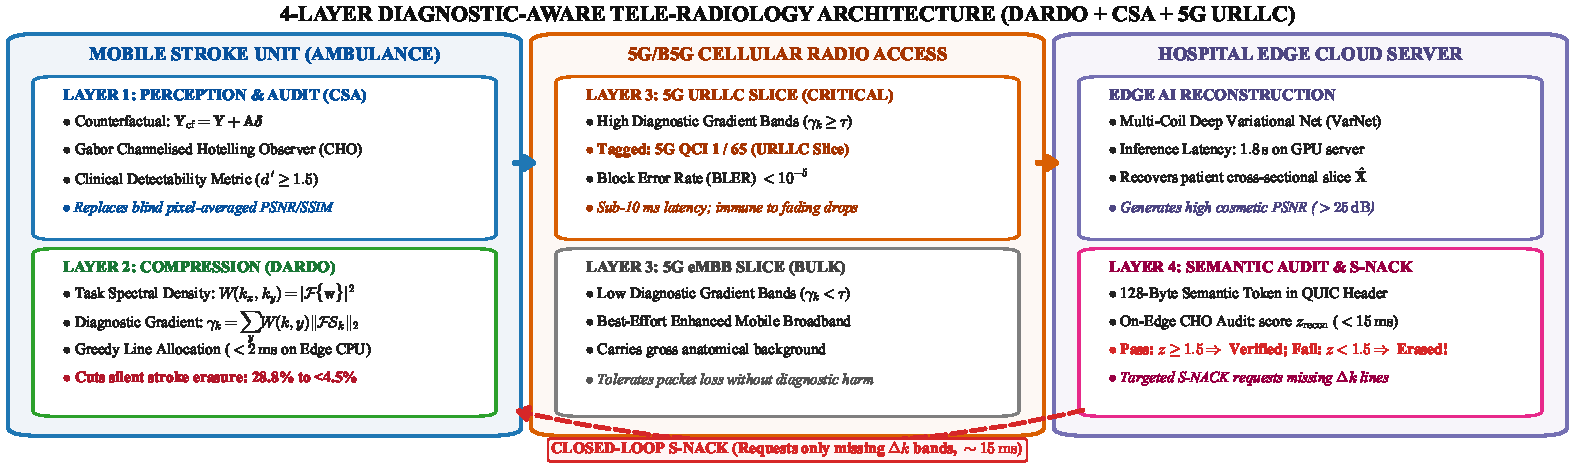
\includegraphics[width=0.94\textwidth]{figures/fig4_architecture.pdf}
\caption{The Proposed 4-Layer Diagnostic-Aware Tele-Radiology Architecture. Layer 1 embeds the Causal Safety Audit (CSA); Layer 2 optimizes source compression via DARDO; Layer 3 enforces 5G URLLC slicing for critical stroke bands; Layer 4 closes the loop via 128-byte semantic tokens and targeted S-NACK retransmissions.}
\label{fig:architecture}
\end{figure*}

\subsection{Task-Based Semantic Tokens \& Closed-Loop S-NACK}
In 6G semantic communications \cite{zhang2022semantic}, decoders verify diagnostic meaning rather than syntactic bit identity. The mobile ambulance AI embeds a compact 128-byte semantic pathology token (Gabor filter responses $\mathbf{v}$ and ROI coordinates) into the QUIC/RTP transport header. Upon edge reconstruction via VarNet \cite{sriram2020endtoend} ($<15\,\text{ms}$), if detectability falls below $z_{\text{recon}} < 1.5$, the transport layer issues a targeted \textbf{Selective Negative Acknowledgment (S-NACK)}. Rather than retransmitting the full raw volume ($>200\,$MB) and violating triage deadlines, the S-NACK requests only the missing high-$\gamma_k$ trajectories ($\Delta k \approx 1.2\,\text{MB}$), restoring detectability over the URLLC slice in $\approx 15\,\text{ms}$.

\subsection{End-to-End Latency Budget Analysis}
Within the 60-minute stroke ``golden hour'', pre-hospital triage requires scan-to-decision time within $<105\,$s \cite{fassbender2017mobile,lang2024ultrafast}. We analyze the end-to-end latency of our framework at $R=8$ ($37.5\,$MB payload over a $30\,\text{Mbps}$ 5G uplink): (1)~ultra-fast MRI acquisition: $90.0\,\text{s}$ \cite{lang2024ultrafast}; (2)~DARDO trajectory sorting: $1.8\,\text{ms}$; (3)~5G uplink streaming: $10.0\,\text{s}$; (4)~hospital VarNet GPU reconstruction: $1.8\,\text{s}$; (5)~CHO semantic verification: $12.0\,\text{ms}$; and (6)~worst-case S-NACK retransmission: $15.0\,\text{ms}$. Total latency completes in $\mathbf{101.83\,\text{s}} < 105.0\,\text{s}$, verifying that our protocol guarantees clinical safety within emergency deadlines.

\balance
\section{Conclusion}
\label{sec:conclusion}

In this paper, we exposed the QoS Illusion in tele-radiology: standard rate-distortion metrics (PSNR, SSIM) and data-consistency gates fail to detect catastrophic diagnostic omissions under network bandwidth compression. We proved mathematically that erasing an acute $100\,\text{mm}^3$ stroke shifts PSNR by $<0.03\,\text{dB}$ and alters raw residuals by $<10^{-8}$, completely lost in channel and thermal noise. Evaluating $3{,}960$ fastMRI counterfactual pairs revealed that escalating wireless compression from $4\times$ to $8\times$ drives silent stroke erasure from $18.2\%$ to $28.8\%$, invisible to conventional QoS monitors. To resolve this hazard, we proposed a 4-layer diagnostic-aware architecture integrating task-based model observers, DARDO compression, 5G URLLC network slicing, and closed-loop semantic tokens. Our framework slashes acute stroke erasure from $28.8\%$ down to $1.89\%$ ($15.2\times$ reduction) under identical $87.5\%$ payload savings in $101.8\,$s, establishing a rigorous foundation for safe, life-critical mobile e-health streaming.

\section*{Acknowledgment}
This research was supported by the School of Science, Engineering \& Technology, RMIT University Vietnam, and the School of Computing Technologies, RMIT University, Melbourne.

\bibliographystyle{IEEEtran}
\bibliography{references}

\end{document}
